% Overleaf: select main.tex, pdfLaTeX, and BibTeX (the default latexmk workflow).
% Generic IEEE journal format. Use the target venue's template before submission.
\documentclass[journal]{IEEEtran}
% For a conference submission, replace the line above with:
% \documentclass[conference]{IEEEtran}

\usepackage{cite}
\usepackage{amsmath,amssymb}
\interdisplaylinepenalty=2500
\usepackage{graphicx}
\usepackage{booktabs,array}
\usepackage{xcolor}
\usepackage{algpseudocode}
\usepackage{tikz}
\usetikzlibrary{arrows.meta,positioning,calc}
\usepackage[hidelinks]{hyperref}
% Keep pending scientific results visible even if editorial notes are hidden.
\newif\ifdraftnotes
\draftnotestrue
\newcommand{\draftnote}[1]{\ifdraftnotes\par\smallskip\noindent\textcolor{red!65!black}{\textbf{Draft note:} #1}\par\smallskip\fi}
\newcommand{\pending}[1]{\ifdraftnotes\textcolor{red!65!black}{\textit{#1}}\else\textit{#1}\fi}
\newcommand{\TBD}{\pending{TBD}}
\newcommand{\taskset}{\mathcal{V}}
\newcommand{\edgeset}{\mathcal{E}}
\newcommand{\nodeset}{\mathcal{N}}
\newcommand{\copies}[1]{\mathcal{P}_{#1}}
\newcommand{\faultset}{\Omega(\chi)}
\newcommand{\cbase}{C^{0}}
\newcommand{\rmax}{R_{\max}}
\newcommand{\reff}{R_{\mathrm{eff}}}
\newcommand{\rhat}{\widehat{R}}
\newcommand{\pos}[1]{\left[#1\right]_{+}}
\DeclareMathOperator{\Pred}{pred}
\DeclareMathOperator{\MLP}{MLP}
\newtheorem{proposition}{Proposition}
\newcommand{\includefinalfigure}[2]{\IfFileExists{#1}{\includegraphics[width=\columnwidth]{#1}}{\pending{#2}}}


\title{GCN-Guided Adaptive Large Neighborhood Search for Recovery-Latency-Constrained Workflow Scheduling in the Computing Continuum}
\author{Author names and affiliations to be added}

\begin{document}
\maketitle

\begin{abstract}
Workflow deployments across cloud, edge, and device resources must balance
execution cost against both application deadlines and the disruption caused by
failures. A deployment that completes before its deadline can still leave
insufficient time for recovery. This paper studies recovery-latency-constrained
hybrid fault-tolerant scheduling of directed acyclic graph workflows. The
decision combines task placement, selective active replication, and passive
reexecution under a deterministic recovery policy. Feasibility couples the
nominal makespan with the largest additional delay over an explicitly defined
set of task-copy, node, and communication-failure scenarios. We develop
GCN-ALNS, a graph-convolution-guided adaptive large neighborhood search that
uses a feasibility-first objective, diversified initialization, and stagnation
restarts. A supervised resource-graph scorer guides construction and repair,
while an exhaustive scenario verifier determines whether an incumbent may be
reported as feasible. Protection modes follow a recovery-aware heuristic,
while learned placement scores also rank replica destinations. The independent
evaluation protocol separates demonstration generation, model selection, and
held-out comparisons across three problem scales, and measures feasibility,
cost, recovery margin, and search effort through paired instance-level
analysis.
\end{abstract}

\begin{IEEEkeywords}
Workflow scheduling, fault tolerance, recovery latency, computing continuum,
graph convolutional networks, adaptive large neighborhood search.
\end{IEEEkeywords}

\section{Introduction}
\label{sec:introduction}
\IEEEPARstart{W}{orkflow} applications express dependencies among processing
tasks and expose opportunities for parallel execution on heterogeneous
resources. Deploying such applications across cloud, edge, and device tiers
creates a placement problem in which execution speed, communication delay,
resource availability, and monetary cost interact. A low-cost node can be an
attractive execution target but a poor recovery destination. Similarly, adding
replicas can reduce the need for reexecution while increasing compute charges,
communication charges, and contention for limited deployment capacity.

An application deadline alone does not describe the disruption that a user is
willing to tolerate. Consider a workflow with deadline $D$, nominal makespan
$\cbase$, and an additional delay $R$ caused by recovery. Meeting the deadline
after a failure requires $\cbase+R\leq D$. A separate recovery service-level
agreement (SLA) may also require $R\leq R_{\mathrm{SLA}}$. Consequently, the
deployment has only
\begin{equation}
  \reff=\min\{R_{\mathrm{SLA}},D-\cbase\}
  \label{eq:intro_budget}
\end{equation}
seconds of effective recovery budget. A cost-minimizing deployment that uses
almost all of $D$ for nominal execution can violate the recovery requirement
even when the declared recovery window appears generous. Conversely, a fast
nominal schedule does not guarantee inexpensive or rapid recovery when its
tasks depend on vulnerable resources or communication paths.

This coupling motivates \emph{joint} placement and fault-tolerance decisions.
Active replication runs multiple task copies and allows a surviving copy to
complete the task. Passive protection deploys one copy and reexecutes affected
work after failure. Choosing a single strategy for every task overlooks
differences in task criticality, slack, communication demand, and replica
placement opportunities. The scheduling decision must therefore account for
both the nominal deployment and the recovery behavior induced by that
deployment.

Classical heterogeneous workflow heuristics, including HEFT and PEFT, provide
useful starting points for makespan-oriented scheduling
\cite{topcuoglu2002heft,arabnejad2014peft}. Reliability-aware and hybrid
fault-tolerant methods introduce replication or reexecution decisions
\cite{qin2023ramoma,taghinezhad2025recrd,ren2026hfwpf}. Their original objectives
and system assumptions, however, are not identical to a joint deadline and
recovery-delay constraint. A comparison must distinguish an algorithmic
design from the simulator, resource model, and failure model under which it is
evaluated. In particular, a common feasibility checker is necessary for
consistent comparisons, but sharing a checker does not by itself make
adaptations equivalent to their original algorithms.

We study a static, single-workflow deployment problem on a fixed computing
continuum. Tasks are placed under cumulative CPU and memory deployment
constraints, active replicas are separated by fault domain during
construction, and a deterministic recovery policy handles an explicitly
enumerated scenario set. We refer to this formulation as the
\emph{recovery-latency-constrained hybrid fault-tolerant scheduling problem}
(RLC-HFTSP). Its scenario model fixes failure locations and times; the
resulting feasibility claim applies to those scenarios rather than every
possible failure time in a physical system.

To solve this problem, we develop GCN-ALNS. Adaptive large neighborhood search
(ALNS) provides the combinatorial search framework
\cite{ropke2006alns,pisinger2007general}. Before a verified feasible deployment
is available, the search prioritizes estimated constraint violations. After
feasibility is established, it emphasizes cost. A graph convolutional network
(GCN) learns placement preferences from feasible solver demonstrations
\cite{kipf2017gcn}. Importantly, the GCN encodes a resource graph; workflow
structure enters through task features. Its scores guide search actions, while
the recovery verifier retains responsibility for certifying incumbents.

The contributions are as follows.
\begin{itemize}
  \item We formulate a deployment-dependent recovery budget that links nominal
  completion, a recovery SLA, and the largest additional delay over a finite
  fault-scenario set. The model specifies compute, communication, passive
  reserve, and recovery-delay cost components without double-counting replica
  compute cost.
  \item We design a feasibility-first ALNS solver with diversified
  initialization, adaptive operators, and stagnation restarts, and integrate
  supervised resource-graph guidance into construction, insertion, and
  destruction, including preference-based ranking of replica destinations.
  \item We establish an independent evaluation protocol that separates
  teacher generation, model selection, and held-out testing. It includes
  shared scenario verification, documented baseline adaptations, paired
  instance-level analysis, and versioned deployment artifacts.
\end{itemize}

The empirical questions concern whether learned guidance changes feasible
solution quality and search effort, which mechanisms account for those
changes, and how these effects vary with workflow scale and SLA tightness.
The manuscript does not assume that the complete solver must dominate every
alternative on every metric.

\section{Related Work}
\label{sec:related_work}
\subsection{Heterogeneous Workflow Scheduling}
HEFT combines task prioritization with resource selection based on estimated
finish times, while PEFT uses optimistic downstream costs to improve
placement decisions \cite{topcuoglu2002heft,arabnejad2014peft}. These methods
remain relevant as low-overhead references and initial-solution generators.
Our implementation fixes the evaluator's per-node order to a canonical
topological replay and does not optimize task order or insert tasks into idle
gaps. Accordingly, the HEFT/PEFT-style baselines in our experiments should be
understood as adaptations to this deployment evaluator, rather than a claim
to reproduce every scheduling freedom of their original formulations.

\subsection{Reliability and Hybrid Fault Tolerance}
RA-MOMA studies reliability-aware multi-objective workflow scheduling in a
multi-cloud setting using memetic search \cite{qin2023ramoma}. RECR-D addresses
fault-tolerant cost-efficient scheduling for energy- and deadline-constrained
IoT workflows in an edge--cloud continuum \cite{taghinezhad2025recrd}. HFWPF
considers hybrid fault tolerance with performance-fluctuating cloud resources
\cite{ren2026hfwpf}. These studies motivate the use of selective replication,
reexecution, and problem-specific placement decisions. They also differ in
energy modeling, resource elasticity, execution-time uncertainty, reliability
objectives, and online behavior.

The present study focuses on a different constraint: recovery must fit both
an explicit delay limit and the deadline slack left by the chosen nominal
deployment. We adapt the placement and protection mechanisms of selected
methods to a common static evaluator and describe the removed or remapped
features in Section~\ref{sec:baselines}. In particular, an adapted method's
behavior under our recovery-delay gate cannot establish that the original
method is inferior on its original problem. This distinction is essential
when the adaptation removes an uncertainty model or an online decision stage
that is central to the source method.

\subsection{Large Neighborhood Search and Learned Guidance}
ALNS extends large neighborhood search by adjusting the selection weights of
multiple destroy and repair operators according to their observed search
outcomes \cite{ropke2006alns,pisinger2007general}. This makes it suitable for
combining placement, replica, and protection-mode changes without enumerating
the entire deployment space. Our solver adds an explicit feasibility-first
phase and uses full scenario verification selectively when considering
feasible incumbents.

GCNs learn node representations through normalized graph propagation
\cite{kipf2017gcn}. Here, the resource graph represents communication-based
proximity among continuum nodes. The learned score estimates the preference
of a task--node assignment under solver demonstrations; it is not an
independent proof of feasibility or an estimate of a globally optimal
assignment. Training is supervised rather than reinforcement-based, and the
score table remains fixed throughout the search for a given instance. The
research question is whether this offline prior improves an already
constraint-aware search under independent evaluation.

\subsection{Workflow Data and External Validity}
WfCommons provides workflow instances and generators that support research
with realistic application characteristics \cite{coleman2022wfcommons}.
The experiments specified in this manuscript currently use custom synthetic
generators whose schemas and broad workflow shapes are inspired by
established scientific workflows and cluster-resource traces. They do not use
real WfCommons executions or raw Alibaba machine traces. Existing parsers and
planned data integration are therefore implementation capabilities, not
evidence that the present experimental instances are trace-driven.

\section{System Model and Problem Formulation}
\label{sec:model}
\begin{table}[!t]
\caption{Principal notation}
\label{tab:notation}
\centering
\footnotesize
\begin{tabular}{@{}p{0.23\columnwidth}p{0.70\columnwidth}@{}}
\toprule
Symbol & Meaning \\
\midrule
$G=(\taskset,\edgeset)$ & Workflow DAG and dependency edges \\
$\nodeset$, $g_k$ & Resource nodes and node $k$'s fault domain \\
$w_i,\sigma_i,\mu_i$ & Task workload, CPU demand, and memory demand \\
$c_k,u_k,q_k$ & Compute speed, background load, and recovery queue estimate \\
$x_{ik},y_i$ & Copy-placement indicator and active-replication mode \\
$\copies{i}$ & Nodes hosting copies of task $i$ \\
$p_{ik},\tau_{k\ell}(d)$ & Execution time and transfer delay \\
$D,R_{\mathrm{SLA}}$ & Deadline and declared recovery-delay limit \\
$\cbase,C^{\omega}$ & Nominal and scenario-specific makespan \\
$\rmax,\reff$ & Largest additional delay and effective recovery budget \\
$h_i,s_{ik}$ & Structural task criticality and learned placement score \\
$\rhat,V$ & Recovery surrogate and estimated violation \\
\bottomrule
\end{tabular}
\end{table}

\subsection{Workflow and Computing Continuum}
A workflow is a DAG $G=(\taskset,\edgeset)$. Task $i$ has workload $w_i$,
CPU demand $\sigma_i$, and memory demand $\mu_i$. Dependency $(i,j)$ carries
data volume $d_{ij}$. The resource set $\nodeset$ is partitioned into cloud,
edge, and device tiers. Node $k$ has compute speed $c_k$, CPU capacity $C_k$,
memory capacity $M_k$, background utilization $u_k$, unit compute price
$\rho_k$, failure-rate parameter $\lambda_k$, and fault-domain label $g_k$.
Its residual deployment capacities are
\begin{equation}
 \overline C_k=C_k(1-u_k),\qquad
 \overline M_k=M_k(1-u_k).
\end{equation}
Execution time is deterministic: $p_{ik}=w_i/c_k$. For different nodes,
\begin{equation}
 \tau_{k\ell}(d)=L_{k\ell}+d/B_{k\ell},\qquad k\ne\ell,
\end{equation}
where $L_{k\ell}$ and $B_{k\ell}$ are link latency and bandwidth. A small
configured local-access delay is used when $k=\ell$. The continuum is fixed
for a scheduling instance; elastic node provisioning, energy consumption,
and stochastic execution-time fluctuations are outside this model.

\subsection{Placement and Protection Modes}
Let $x_{ik}\in\{0,1\}$ indicate whether task $i$ has a copy on node $k$, and
let $y_i\in\{0,1\}$ denote its protection mode. Passive tasks have one
deployed copy and can be reexecuted after failure. Active tasks have multiple
concurrently provisioned copies. Define
$\copies{i}=\{k:x_{ik}=1\}$ and impose
\begin{equation}
 1+y_i\leq \sum_k x_{ik}
 \leq 1+(m_{\max}-1)y_i.
 \label{eq:replicas}
\end{equation}
The implementation uses $m_{\max}=2$, so an active task has exactly two
copies. For each fault domain $g$, construction enforces
\begin{equation}
 \sum_{k:g_k=g}x_{ik}\leq 1.
 \label{eq:domains}
\end{equation}
This is a replica-separation requirement. It does not imply that the default
verification set includes whole-domain outages.

The capacity model constrains the cumulative footprint of deployed task
copies:
\begin{align}
 \sum_i\sigma_i x_{ik}&\leq\overline C_k, & k&\in\nodeset,\\
 \sum_i\mu_i x_{ik}&\leq\overline M_k, & k&\in\nodeset.
 \label{eq:capacity}
\end{align}
These inequalities reserve deployment resources across tasks; they are not
instantaneous resource constraints that release capacity after every task
completion. This assumption is maintained during recovery placement, which
starts from the original deployment footprint and adds reexecution demand.

\subsection{Nominal Schedule Evaluation}
The evaluator traverses tasks in a deterministic topological order and
serializes their copies on each node. With $a_k$ denoting node availability,
the data-ready time of copy $(i,k)$ is
\begin{equation}
 b_{ik}=\max_{j\in\Pred(i)}\min_{q\in\copies{j}}
       \{f_{jq}+\tau_{qk}(d_{ji})\},
 \label{eq:data_ready}
\end{equation}
where an empty predecessor maximum is zero. Start and finish times follow
\begin{equation}
 s_{ik}=\max\{a_k,b_{ik}\},\quad f_{ik}=s_{ik}+p_{ik},\quad a_k\leftarrow f_{ik}.
 \label{eq:nominal_schedule}
\end{equation}
Task completion uses the earliest copy,
\begin{equation}
 F_i=\min_{k\in\copies{i}}f_{ik},\qquad \cbase=\max_i F_i.
 \label{eq:nominal_makespan}
\end{equation}
Copies contribute their full modeled compute and communication charges even
when another copy completes earlier. Task-order optimization and idle-gap
insertion are not decision variables of the implemented evaluator.

\subsection{Controllable Fault Scenarios}
The default scenario set depends on the deployment:
\begin{equation}
 \faultset=\Omega^{\mathrm{copy}}(\chi)\cup
 \Omega^{\mathrm{node}}(\chi)\cup\Omega^{\mathrm{link}}(\chi).
 \label{eq:fault_set}
\end{equation}
It contains one copy-failure scenario for every deployed copy and one
node-failure scenario for every occupied node. For each workflow edge whose
effective producer and consumer execute on different nodes, it also includes
an associated transfer-failure scenario. Effective nodes are determined by
the earliest nominal copies in~\eqref{eq:nominal_makespan}; the default set
does not enumerate every possible replica-to-replica transfer failure.

Scenario times are prescribed from the nominal schedule. A copy fails at its
planned finish time; a node fails at its first planned task start; a transfer
fails at its planned completion. Only one such event is injected in a
scenario. Correlated domain failures can be evaluated separately but are not
part of~\eqref{eq:fault_set}. Thus, the term ``worst case'' below means the
largest delay within this explicit, finite scenario set. It does not quantify
over arbitrary failure times, all combinations of failures, or all physical
communication events.

\subsection{Deterministic Recovery Policy}
For each $\omega\in\faultset$, the simulator performs a fault-aware forward
replay in the same topological order. A directly affected active task with
healthy copies completes according to
\begin{equation}
 F_i^{\omega}=\min_{k\in\mathcal H_i^{\omega}}
 \max\{\widetilde f_{ik}^{\omega},
       t_{\omega}+\delta_d+\delta_s+\delta_{\mathrm{sync}}\},
 \label{eq:active_recovery}
\end{equation}
where $\mathcal H_i^{\omega}$ contains surviving copies and
$\widetilde f_{ik}^{\omega}$ is the copy finish time in the replay.
The constants represent detection, switching, and synchronization delay.

When no usable copy remains, a healthy node $k'$ is selected for reexecution.
It must satisfy residual footprint constraints and the policy's domain
restrictions. If no such node exists, the scenario makespan is infinite.
Otherwise,
\begin{equation}
\begin{split}
 F_i^{\omega}={}&\max\{b_{ik'}^{\omega},a_{k'}^{\omega},
                 t_{\omega}+\delta_d+\delta_r\}\\
               &+q_{k'}+p_{ik'},
\end{split}
\label{eq:passive_recovery}
\end{equation}
where $\delta_r$ is replanning delay and $q_{k'}$ is a configured recovery
queue estimate. Node availability $a_{k'}^{\omega}$ includes both healthy
tasks already replayed and earlier reexecutions; omitting it would allow
overlapping execution on a serialized node. Recovery input routing uses the
effective predecessor retained by the replay. This differs from nominal
input selection over all predecessor copies in~\eqref{eq:data_ready}.

Recovery-node selection minimizes a configured heuristic:
\begin{equation}
\begin{split}
 Q_i(k)={}&\theta_1q_k+
 \theta_2\sum_{j\in\Pred(i)}\tau_{\kappa_j k}(d_{ji})
 +\theta_3p_{ik}\\
 &+\theta_4h_i(1-e^{-\lambda_kp_{ik}})
 +\theta_5\rho_kp_{ik},
\end{split}
\label{eq:recovery_selection}
\end{equation}
where $\kappa_j$ is the recovered effective node of predecessor $j$, and
$h_i\in[0,1]$ is structural criticality. Link failures introduce a configured
wait and retransmission delay before affected input becomes available.
This deterministic policy is part of the evaluator, not an optimal recovery
schedule computed independently for each deployment.

\subsection{Recovery SLA and Effective Budget}
Let $C^{\omega}$ be the replay makespan. Define
\begin{equation}
 R_{\omega}=\pos{C^{\omega}-\cbase},\qquad
 \rmax=\max_{\omega\in\faultset}R_{\omega}.
 \label{eq:recovery_delay}
\end{equation}
A complete, capacity-feasible deployment must satisfy
\begin{equation}
 \cbase\leq D,\qquad
 \rmax\leq\reff=\min\{R_{\mathrm{SLA}},D-\cbase\}.
 \label{eq:sla}
\end{equation}
Its recovery safety margin is $M(\chi)=\reff-\rmax$.
Figure~\ref{fig:budget} illustrates why nominal slack and recovery tolerance
must be considered together.

\begin{proposition}
For a complete, capacity-feasible deployment and the specified scenario set,
\eqref{eq:sla} holds if and only if $\cbase\leq D$, every
$C^{\omega}\leq D$, and every $R_{\omega}\leq R_{\mathrm{SLA}}$.
\end{proposition}
\begin{IEEEproof}
If~\eqref{eq:sla} holds, then
$C^{\omega}\leq\cbase+\rmax\leq D$ and
$R_{\omega}\leq\rmax\leq R_{\mathrm{SLA}}$.
Conversely, $C^{\omega}\leq D$ and $\cbase\leq D$ imply
$R_{\omega}\leq D-\cbase$. Combining this with the recovery SLA and taking
the maximum over scenarios gives~\eqref{eq:sla}.
\end{IEEEproof}

\begin{figure}[!t]
 \centering
 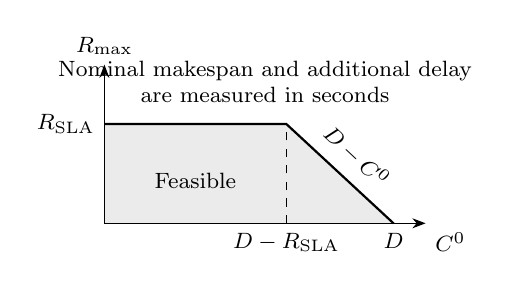
\begin{tikzpicture}[x=0.68cm,y=0.63cm,>=Stealth,font=\footnotesize]
 \fill[gray!16] (0,0)--(5.4,0)--(3.4,2.0)--(0,2.0)--cycle;
 \draw[->] (0,0)--(6.0,0) node[below right] {$\cbase$};
 \draw[->] (0,0)--(0,3.2) node[above] {$\rmax$};
 \draw[thick] (0,2.0)--(3.4,2.0)--(5.4,0);
 \draw[dashed] (3.4,0)--(3.4,2.0);
 \node[left] at (0,2.0) {$R_{\mathrm{SLA}}$};
 \node[below] at (5.4,0) {$D$};
 \node[below] at (3.4,0) {$D-R_{\mathrm{SLA}}$};
 \node at (1.7,0.85) {Feasible};
 \node[rotate=-43,above] at (4.45,1.05) {$D-\cbase$};
 \node[align=center] at (3.0,2.85) {Nominal makespan and additional delay\\are measured in seconds};
\end{tikzpicture}

 \caption{Conceptual feasible timing region. The effective recovery limit is
 the smaller of the declared window and the remaining deadline slack. This
 diagram illustrates the model; it is not an experimental plot.}
 \label{fig:budget}
\end{figure}

\subsection{Cost Objective}
The monetary component of nominal deployment is
\begin{align}
 J_{\mathrm{comp}}&=\sum_i\sum_{k\in\copies{i}}\rho_kp_{ik},\\
 J_{\mathrm{comm}}&=\gamma_c\sum_{(i,j)\in\edgeset}d_{ij}
      \sum_{k\in\copies{i}}\sum_{\ell\in\copies{j}}\mathbf1[k\ne\ell],\\
 J_{\mathrm{res}}&=\gamma_{\mathrm{res}}\sum_{i:y_i=0}\sigma_i.
 \label{eq:cost_terms}
\end{align}
Communication billing counts all provisioned cross-node replica pairs, even
though input readiness uses the fastest nominal predecessor copy. This is an
explicit billing convention. Replica compute is already included in
$J_{\mathrm{comp}}$ and is not added again as a separate backup charge.

Let $J_0=J_{\mathrm{comp}}+J_{\mathrm{comm}}+J_{\mathrm{res}}$. The reported
objective adds a recovery-delay proxy:
\begin{equation}
 J(\chi)=J_0(\chi)+\gamma_{\omega}\overline R(\chi),\qquad
 \overline R=\frac{1}{|\faultset|}\sum_{\omega\in\faultset}R_{\omega}.
 \label{eq:objective}
\end{equation}
For feasible deployments, all terms of this average are finite. It is a
uniform scenario-average delay with a configured conversion weight, not a
probability-weighted expected financial loss. We use it for feasible-solution
comparison and do not interpret the simulator's finite-value proxy on
unrecoverable deployments as an expectation.

RLC-HFTSP minimizes~\eqref{eq:objective} over placement and protection modes
subject to~\eqref{eq:replicas}--\eqref{eq:capacity}, nominal dependency
evaluation, and~\eqref{eq:sla}. The recovery policy is fixed. The problem is
a combinatorial deployment search; no claim of global optimality or an
unproved complexity reduction is required by the proposed heuristic.

\section{GCN-Guided Adaptive Large Neighborhood Search}
\label{sec:method}
\subsection{Search Architecture}
GCN-ALNS separates three roles: learned assignment preferences, inexpensive
search guidance, and full scenario verification. Figure~\ref{fig:overview}
shows this separation. The learned component ranks candidate placements; it
does not replace the recovery simulator or alter the SLA definition.

For a candidate deployment, the quick evaluator computes its nominal
schedule, deployment cost $J_0$, and an approximate recovery-delay surrogate
$\rhat$. The surrogate takes the largest positive difference between a
task-local recovery estimate and that task's schedule slack. For an active
task, the local estimate includes detection, switching, synchronization, and
the finish-time gap between its two copies. For a passive task, it includes
detection, replanning, a queue estimate, incoming communication, and
reexecution. This approximation does not enumerate~\eqref{eq:fault_set} and
is not a proven upper bound on $\rmax$.

Define estimated violation and penalized cost as
\begin{align}
 V(\chi)&=\pos{\cbase-D}+\pos{\rhat-\reff},\\
 \Phi(\chi)&=J_0(\chi)+\eta_D\pos{\cbase-D}
                     +\eta_R\pos{\rhat-\reff}.
 \label{eq:quick_objective}
\end{align}
Before a fully verified feasible solution has been found, the search
minimizes $V+\epsilon J_0$, with $\epsilon=10^{-4}$ providing a small cost
preference. It switches to $\Phi$ after establishing feasibility. This
mechanism distinguishes the search's constraint-reduction phase from its
cost-reduction phase.

Full verification is reserved for candidates that the surrogate regards as
feasible and whose quick deployment cost is below the stored feasible
solution's reported score. If a candidate passes exhaustive scenario
enumeration, the feasible-solution register is updated with its deployment
and full cost. The quick screen uses $J_0$, whereas the stored score includes
the recovery proxy in~\eqref{eq:objective}; the resulting heuristic is not a
monotone descent method for the full reported objective. Moreover, an
overconservative surrogate can screen out an actually feasible deployment.
We therefore claim neither search completeness nor an optimality guarantee.

\begin{figure*}[!t]
 \centering
 \resizebox{0.97\textwidth}{!}{%
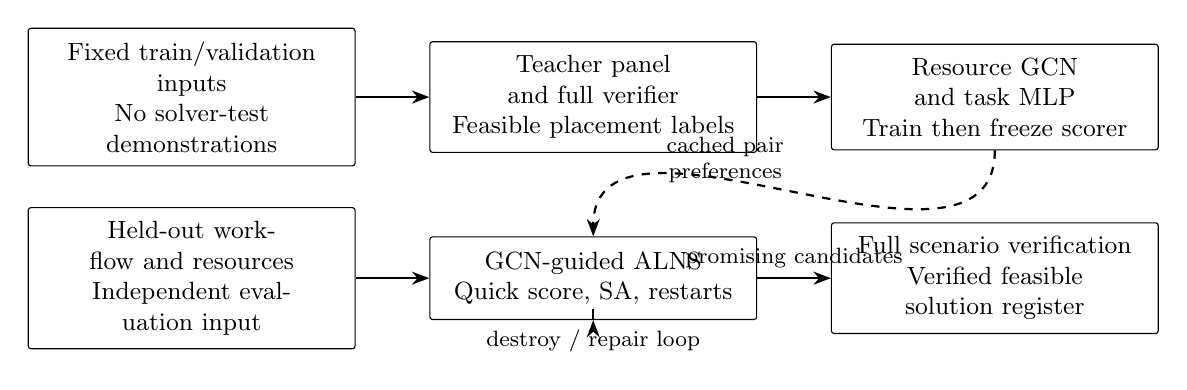
\begin{tikzpicture}[
 box/.style={draw,rounded corners=1pt,align=center,text width=3.8cm,
             minimum height=1.05cm,inner sep=5pt},
 arr/.style={-{Stealth[length=2.2mm]},thick},
 font=\small]
 \node[box] (train) at (0,2.3) {Fixed train/validation inputs\\No solver-test demonstrations};
 \node[box] (teacher) at (5.1,2.3) {Teacher panel and full verifier\\Feasible placement labels};
 \node[box] (model) at (10.2,2.3) {Resource GCN and task MLP\\Train then freeze scorer};
 \node[box] (test) at (0,0) {Held-out workflow and resources\\Independent evaluation input};
 \node[box] (search) at (5.1,0) {GCN-guided ALNS\\Quick score, SA, restarts};
 \node[box] (verify) at (10.2,0) {Full scenario verification\\Verified feasible solution register};
 \draw[arr] (train)--(teacher);
 \draw[arr] (teacher)--(model);
 \draw[arr] (test)--(search);
 \draw[arr] (search)--node[above,font=\footnotesize]{promising candidates}(verify);
 \draw[arr,dashed] (model.south) to[out=-90,in=90]
    node[above left,font=\footnotesize,align=center]{cached pair\\preferences}(search.north);
 \draw[arr] (search.south) to[out=-115,in=-65,looseness=3]
    node[below,font=\footnotesize]{destroy / repair loop}(search.south);
\end{tikzpicture}%
}

 \caption{Training and deployment workflow. Only fixed train/validation
 instances provide teacher demonstrations. The frozen scorer supplies
 preferences to ALNS on a held-out instance. A quick evaluator guides search,
 while full scenario enumeration determines whether a feasible solution may
 be retained. The resource GCN and task MLP are separate encoders.}
 \label{fig:overview}
\end{figure*}

\subsection{Initialization, Operators, and Restarts}
Initial solutions include a criticality-based hybrid deployment and an
earliest-finish-time deployment. When learned guidance is enabled, a GCN-led
greedy construction is added. Candidates are ranked by estimated feasibility,
violation, and penalized objective.

The destroy pool contains random removal, critical-task removal, high-risk
removal, congested-node removal, and removal of excessive backups. A learned
operator additionally targets tasks placed on low-scoring nodes. Five repair
operators emphasize normalized insertion cost, recovery delay, monetary cost,
active-copy enhancement, or passive-mode conversion. Removing and repairing
tasks changes both deployment locations and the conditions under which a
task receives replicas.

Destroy and repair operators are sampled by weighted roulette. Segment-level
updates combine their previous weights with rewards for accepted, improving,
or best-search outcomes. A candidate with a worse current search score can
still be accepted with simulated-annealing probability
\begin{equation}
 P_{\mathrm{acc}}=\exp\!\left(-\frac{S(\chi')-S(\chi)}{T}\right),
 \label{eq:sa}
\end{equation}
where $S$ is the active feasibility-first or penalized score, and the
temperature decreases geometrically. At prolonged stagnation, the solver
destroys and repairs a larger portion of a reference deployment, resets the
temperature, and consumes one of a bounded number of restarts. If the restart
budget is exhausted, it can stop before the iteration limit.

% IEEEtran uses a figure float for pseudocode instead of a dedicated
% algorithm float. algpseudocode supplies only the pseudocode layout.
\begin{figure}[!t]
\centering
\begin{minipage}{\columnwidth}
\hrule\vspace{3pt}
\footnotesize
\begin{algorithmic}[1]
\Require Workflow/resource instance, parameters, iteration limit $B$
\State Compute structural features and cached learned scores
\State Construct diverse initial solutions; select current $\chi$
\State Initialize operator weights, temperature, and restart budget
\State $\chi_F\gets\varnothing$; $J_F\gets+\infty$
\If{the quick screen accepts the initial solution}
  \State Fully verify it; set $\chi_F\gets\chi$, $J_F\gets J(\chi)$ if feasible
\EndIf
\For{$t=1,\ldots,B$}
  \State Select destroy and repair operators by adaptive roulette
  \State $\chi'\gets\operatorname{Repair}(\operatorname{Destroy}(\chi))$
  \State Evaluate $J_0$, nominal timing, $\rhat$, and $V$ for $\chi'$
  \State Use $V+\epsilon J_0$ until $\chi_F$ exists, then use $\Phi$
  \State Accept $\chi'$ into the current search state by improvement or SA
  \If{quick-feasible$(\chi')$ and $J_0(\chi')<J_F$}
    \State Enumerate all $\omega\in\Omega(\chi')$ with the shared verifier
    \If{$\chi'$ passes the full capacity and recovery gate}
      \State $\chi_F\gets\chi'$; $J_F\gets J(\chi')$
    \EndIf
  \EndIf
  \State Accumulate operator rewards; update weights at segment boundaries
  \If{stagnation threshold is reached}
    \State If permitted, restart with a large destroy/repair step; otherwise stop
    \State Evaluate the restart and apply the same feasible-register check
  \EndIf
\EndFor
\State \Return $\chi_F$ if present; otherwise return the best quick-search state
\end{algorithmic}
\vspace{3pt}\hrule
\end{minipage}
\caption{GCN-ALNS search procedure with a shared recovery verifier.}
\label{alg:gcnalns}
\end{figure}

\subsection{Resource-Graph Scoring Network}
The physical resource graph connects each node to its $k$ nearest neighbors
under unit-data communication delay, then symmetrizes the edges. With
$\widetilde A=A+I$ and its degree matrix $\widetilde D$, propagation uses
\begin{equation}
 H^{(\ell+1)}=\widetilde D^{-1/2}\widetilde A\widetilde D^{-1/2}
                  \bigl(H^{(\ell)}W^{(\ell)}+b^{(\ell)}\bigr),
 \label{eq:gcn}
\end{equation}
with ReLU and dropout between graph layers. Node inputs combine 12 resource
features with a learned fault-domain embedding. A separate MLP maps 12 task
features---including workload, rank, slack, degree, level, and structural
criticality---to a task embedding. No graph convolution is performed on the
workflow DAG itself.

Scalar criticality combines normalized upward rank, inverse structural slack,
and out-degree:
\begin{equation}
 h_i=\vartheta_1\widetilde{\mathrm{rank}}_i+
 \vartheta_2\widetilde{(\mathrm{slack}_i+\varepsilon)^{-1}}+
 \vartheta_3\widetilde{\mathrm{outdeg}}_i,
\end{equation}
with weights $(0.4,0.4,0.2)$ in the registered configuration. Structural
features are computed from average execution and communication estimates
before choosing a deployment.

For task $i$ and node $k$, a nine-dimensional interaction vector $z_{ik}$
contains execution time, a node-risk feature, a local recovery-risk proxy,
deployment cost, communication affinity, a compute-speed ratio, and three
resource/deadline compatibility indicators. The placement preference is
\begin{equation}
 s_{ik}=\operatorname{sigmoid}\!\left(
 \MLP([h_i^{T},h_k^{N},h_i^{T}\odot h_k^{N},z_{ik}])\right).
 \label{eq:placement_score}
\end{equation}
Here $h_i^{T}$ is a task embedding and must not be confused with scalar
criticality $h_i$. Predictions for all task--node
pairs are computed once and cached; they do not change with the partial
deployment during an ALNS run.

\subsection{Integrating the Learned Preferences}
For a task's current candidate node set, each insertion component is
min--max normalized within that set. Insertion minimizes
\begin{equation}
\begin{split}
 I_{ik}={}&\alpha_1\widetilde{\mathrm{ECT}}_{ik}
 +\alpha_2\widetilde{\mathrm{Cost}}_{ik}
 +\alpha_3\widetilde{\mathrm{Risk}}_{ik}\\
 &+\alpha_4\widetilde{\mathrm{RecRisk}}_{ik}
 +\alpha_5\widetilde{\mathrm{Load}}_{ik}
 -\alpha_6 h_i\widetilde s_{ik}.
\end{split}
\label{eq:insertion}
\end{equation}
Normalization also applies to the learned score. Candidate screening checks
resource capacity, relevant domain exclusions, and an estimated task finish
against the deadline. It does not establish a hard recovery-delay bound. A
fallback can still construct a candidate when screening finds no node, which
is another reason that final verification is necessary.

The learned scorer influences the greedy initial construction and the
low-score destroy operator as well as~\eqref{eq:insertion}. Replica selection
can also use its node preferences. Repair chooses active replication when a
local recovery estimate exceeds the effective budget. The final method
combines this heuristic protection rule with a learned placement scorer.
Disabling the learned
replica-ranking hook in the component study removes pair-score guidance for
backup destinations while retaining the heuristic protection rule.

\subsection{Learning from Feasible Demonstrations}
A teacher panel runs passive and replicated heuristics together with ALNS on
each designated learning or validation input. Every demonstration is checked
by the same scenario verifier. Among feasible panel outputs, the cheapest
top fraction $\zeta=0.2$ is retained, with at least one output if any is
feasible. Chosen task--node pairs become positive examples. A positive pair
from a demonstration is weighted by
\begin{equation}
 w_{ik}=(1+h_i)\left[1-\frac{\rmax}{\reff}\right]_{[0,1]},
 \label{eq:teacher_weight}
\end{equation}
with the zero-budget case handled separately. Repeated positives retain the
largest associated weight. Unselected compatible nodes provide sampled
contrastive negatives; they are not proven to be invalid assignments in all
possible deployments.

Training combines positive and negative binary cross-entropy with a pairwise
ranking term:
\begin{equation}
\begin{split}
 \mathcal L={}&\mathcal L_{\mathrm{BCE}}^{+}
 +\mathcal L_{\mathrm{BCE}}^{-}
 -\lambda_{\mathrm{rank}}
   \mathbb E_{(i,k^+,k^-)}
   [\overline w_{ik^+}\log\operatorname{sigmoid}(a_{ik^+}-a_{ik^-})],
\end{split}
\label{eq:training_loss}
\end{equation}
where $a_{ik}$ is a placement logit and positive weights are normalized to
mean one within a training batch. The final scorer is selected on the original
validation instances and frozen before held-out testing. Alternative training
configurations are retained as internal development records rather than
presented as separate solver variants.

\subsection{Verification Cost and Practical Limits}
If a deployment has $F$ enumerated faults, verification performs $F$ forward
replays. Each replay can scan the entire node set when selecting recovery
destinations and must evaluate the affected dependencies. The current Python
implementation also performs repeated edge scans when obtaining predecessor
lists; these costs should not be hidden behind a claim of constant-time
dependency lookup. Caching learned scores
avoids repeating a network forward pass at every insertion, but insertion,
schedule evaluation, and full verification can still dominate elapsed time.
Measured runtime and iteration-based search effort are therefore reported
separately.

\section{Experimental Design}
\label{sec:experiments}
\begin{table}[!t]
\caption{Registered experimental settings}
\label{tab:settings}
\centering
\footnotesize
\begin{tabular}{@{}p{0.40\columnwidth}p{0.53\columnwidth}@{}}
\toprule
Setting & Value \\
\midrule
Learning/validation candidates & 60 / 15 instances \\
Feasible demonstration instances & 26 training / 4 validation \\
Held-out instances & 45 small / 30 medium / 15 large \\
Tasks and nodes per instance & 50 / 150 / 500 by scale \\
Workflow families & Montage, CyberShake, Epigenomics, LIGO, SIPHT shapes \\
Task CPU/memory demand & One configured unit each \\
Max. deployed active copies & 2 \\
Detection/replanning delay & 1.0 / 0.5 s \\
Switch/synchronization delay & 0.5 / 0.5 s \\
Link-recovery wait & 2.0 s \\
GCN layers/hidden width & 2 / 64 \\
Domain embedding / neighbors & 8 dimensions / 8 neighbors \\
GCN dropout / learning rate & 0.3 / $10^{-3}$ \\
Adam weight decay & $5\times10^{-4}$ \\
Negatives per positive & 5 \\
Pairwise ranking loss weight & 0.1 \\
Maximum epochs / patience & 100 / 10 \\
ALNS restart budget & 2 \\
Insertion GCN weight & 0.5 \\
Main small/medium budget & 1000 iterations, 10 seeds \\
Main large budget & 800 iterations, 5 seeds \\
\bottomrule
\end{tabular}
\end{table}

\begin{table}[!t]
\caption{SLA settings relative to the nominal HEFT-style reference}
\label{tab:sla}
\centering
\begin{tabular}{lcc}
\toprule
Scenario & $D/T_{\mathrm{ref}}$ & $R_{\mathrm{SLA}}/T_{\mathrm{ref}}$ \\
\midrule
Tight & 1.15 & 0.05 \\
Medium & 1.30 & 0.10 \\
Loose & 1.50 & 0.20 \\
\bottomrule
\end{tabular}
\end{table}

\subsection{Research Questions}
The independent evaluation addresses three questions.
\begin{itemize}
 \item \textbf{RQ1:} How do feasibility, feasible-solution cost, and recovery
 margin compare with nonlearned ALNS and the baseline suite?
 \item \textbf{RQ2:} Which search mechanisms and protection-policy choices
 account for observed changes, and are those changes supported by paired
 analysis?
 \item \textbf{RQ3:} How does learned guidance affect solution quality under
 different iteration budgets, and how does iteration efficiency differ from
 total elapsed time?
\end{itemize}

\subsection{Synthetic Instances and SLA Calibration}
Instances combine five custom DAG-shape generators named after Montage,
CyberShake, Epigenomics, LIGO, and SIPHT workflow families. Runtimes follow a
lognormal distribution with log-space mean 2 and standard deviation 0.7,
while dependency data volumes are sampled from a
configured range of 5--200 MB. These generators approximate broad structural
patterns; they are not real application executions or outputs of the
WfCommons generator. The current synthetic path assigns every task one unit
of CPU demand and one unit of memory demand. Workload heterogeneity therefore
comes primarily from runtime and dependency structure, while resource
capacity varies across nodes.

Synthetic machines draw CPU capacities from $\{8,16,32,64,96\}$ and memory
capacities from $\{16,32,64,128,256\}$. The medium-load setting samples
utilization between 0.30 and 0.60. Quality-based tier assignment combines
capacity, utilization, and variation, followed by tier-dependent prices and
failure-rate parameters. Links use tier-pair latency/bandwidth tables with
deterministic multiplicative perturbations. Fault domains are synthetic
hash-based groups, not observed racks or power domains. Resource data are
cluster-trace-inspired rather than measurements extracted from a production
trace.

For each instance, a passive HEFT-style reference defines
$T_{\mathrm{ref}}$. Deadline and recovery window are scaled as shown in
Table~\ref{tab:sla}. Small, medium, and large instances contain 50, 150, and
500 tasks and the same number of resource nodes, respectively. The held-out
set contains 45, 30, and 15 instances across these scales, for 90 instances
in total. Each SLA setting has 30 test instances across all scales. We do not
retune the SLA parameters after observing the test-set feasibility rates.

\subsection{Independent Learning and Model Selection}
The input protocol fixes 60 learning candidates and 15 validation candidates
before teacher generation. Workflow-content and resource-snapshot hashes
prevent cross-role reuse, including renamed or SLA-modified copies. The
teacher runs only on these inputs and retains an instance only when it finds
at least one verifier-feasible demonstration. In the completed rebuild, 26
training and four validation instances contributed demonstrations. Failed
teacher instances remain assigned to their original roles; they are not
replaced by solver-test instances.

Crucially, supervised-label availability does not redefine the validation or
test population. All 15 original validation instances are retained for
end-to-end solver comparison, including those for which the teacher found
no feasible demonstration. The 90 test instances use separate random-seed
blocks and are never supplied to the teacher or training loss.

Candidate training configurations use the same frozen teacher dataset.
Validation loss controls early stopping.
End-to-end validation uses five repeated solver seeds per instance, with
1000 ALNS iterations as the maximum budget. The registered model-selection
rule first prefers more feasible validation runs. If feasibility ties, it
compares relative cost on identically paired runs where both candidates are
feasible; a remaining tie follows the preregistered candidate priority.
All other search
parameters, including the insertion weight of 0.5, remain fixed.

Validation selected the placement-only checkpoint, with the heuristic
protection rule described in Section~\ref{sec:method}. This single checkpoint
is frozen before testing and used throughout the main, component, and budget
studies. Alternative checkpoints and their diagnostic comparisons are
archived as development records and do not redefine the final model using
test-set outcomes.

\subsection{Baseline Configurations}
\label{sec:baselines}
The suite contains 14 solver labels. Eight built-in labels represent
HEFT-style placement, PEFT-style placement, no-fault-aware placement,
reactive-only placement, full active replication, critical-path replication,
criticality-based hybrid protection, and reliability-aware placement.
HEFT and No-FT share the same passive placement logic in this implementation
and should not be counted as independent algorithmic evidence. Every
returned deployment is evaluated with the same nominal scheduler, recovery
policy, and cost model.

Four additional configurations are external references:
\begin{itemize}
 \item \textbf{RECR-D adaptation:} Retains resource penalties, distributed
 sub-deadlines, and bounded replica promotion. Energy terms are removed;
 placement is performed in the evaluator's canonical order to avoid a
 mismatch between planned and replayed schedules. Recovery-budget feedback
 is mapped to the common simulator rather than the source reliability model.
 \item \textbf{HFWPF adaptation:} Retains the slack-based choice between
 replication and reexecution and a capacity-biased placement rule. The
 source method's execution-time uncertainty, elastic virtual machines, and
 online adaptation are not reproduced.
 \item \textbf{GA-Placement:} Uses a conventional genetic search over placement
 and protection choices as a generic evolutionary reference. It is not a
 reproduction of a genetic-programming hyper-heuristic.
 \item \textbf{RA-MOMA adaptation:} Uses a multi-objective memetic search with
 HEFT-style initialization and problem-specific neighborhoods. The resource
 model is fixed, order genes are omitted, and source reliability and billing
 terms are mapped to the evaluator's cost and recovery-risk objectives.
\end{itemize}
These are explicitly static adaptations, not bit-exact reproductions of
the cited systems \cite{taghinezhad2025recrd,ren2026hfwpf,qin2023ramoma}.
Results under this common gate assess the adapted configurations on
RLC-HFTSP; they do not rank the source papers on their original tasks.
Nonlearned ALNS uses the same search framework as GCN-ALNS, with all learned
hooks disabled.

\subsection{Registered Studies and Computational Budgets}
The main comparison uses ten repeated seeds for stochastic methods on small
and medium instances and five on large instances. The maximum ALNS budgets
are 1000 and 800 iterations, respectively. Deterministic references run once
per instance. The main comparison therefore contains 4200 planned records.
The repeated runs measure optimizer variability on fixed instances; they are
not additional independent workflow samples. Different algorithm families
retain their registered internal search parameters, so the main study is
not a matched-wall-clock comparison across all methods.

The component study uses small and medium test instances, ten repeated
seeds, and 1000 iterations. Its 14 configurations include the complete solver
and removals of learned guidance, warm start, learned replica ranking,
learned destruction, feasibility-first scoring, restarts, initialization
diversity, recovery penalty, deployment risk, domain separation, dynamic
rescheduling, and two repair-mode preference variants. This produces
10\,500 planned records.

These changes belong to different categories. Disabling dynamic rescheduling
restricts reexecution to the task's original domains and changes the recovery
policy; it does not eliminate recovery. Removing domain separation relaxes
an admissibility constraint and is not a pure search-operator ablation.
The variants originally labelled all-active and all-passive apply a mode
preference when repairing removed tasks. Initialization and other repair
actions can retain or change modes, so these configurations do not impose a
strict homogeneous policy on every task. Their results describe repair-mode
preferences. A clean comparison of strictly all-active, all-passive, and
hybrid deployments requires globally constrained, separately versioned runs.
These changes must be distinguished from removing learned ranking or a search
restart.

The budget study compares ALNS and GCN-ALNS on small instances at 50, 100,
200, 500, and 1000 iterations, with ten seeds each, yielding 4500 records.
These three studies contain 19\,200 planned records. Their scopes and budgets
are fixed before inspecting the complete test results. Additional
training-configuration diagnostics are archived separately; they are not an
independent research question or a basis for replacing the frozen checkpoint.

\subsection{Metrics and Statistical Analysis}
Primary metrics are SLA-feasible rate, feasible-deployment cost,
$M(\chi)=\reff-\rmax$, and the iteration at which the solver first records a
verified feasible deployment. We also record full solver runtime, final
verification time, one-time learned inference time, replica usage, and
scenario-set size. Reported verification time for an individual result is
the final evaluation call; it does not account for every verification call
inside ALNS. It cannot alone identify the full solver's dominant runtime
component.

Feasible rate is first averaged over repeated seeds for each instance, then
macro-averaged over instances. For the main descriptive cost table, feasible
seeds are first averaged within each instance, then instances with at least
one feasible run receive equal weight. These method-specific cost means are
descriptive because their successful instance sets can differ. Comparative
cost, recovery margin, and first-feasible iteration are paired by the same
instance and seed and restricted to runs where both methods succeed; unknown
first-feasible iteration markers are excluded. Pairwise differences are then
aggregated within instances so the workflow instance, rather than every
optimizer seed, is the independent statistical unit.

We report paired mean differences, 95\% instance-bootstrap intervals with
2000 resamples, paired $t$-tests, and Wilcoxon signed-rank tests where defined.
For the component comparisons, Holm adjustment is performed separately for
each reported metric family. A feasibility increase, a lower cost among
different successful subsets, and a higher conditional safety margin are
not interchangeable findings. Likewise, fewer iterations to feasibility
must not be presented as a directly measured reduction in wall-clock
time-to-feasibility.

\subsection{Execution Environment and Reproducibility}
The current run uses Windows 11, Python 3.12.4, NumPy 1.26.4, and PyTorch
2.5.1 with CUDA 12.1 on one NVIDIA A40 GPU. The host exposes 32 logical CPU
processors. GPU execution is used for training; per-instance score inference
in the scheduling pipeline is performed on CPU. Independent solver runs use
eight worker processes for ordinary stages and 12 for the large main study,
with per-worker numerical-library threads limited to one.

The insertion weights in~\eqref{eq:insertion} are
$(1,0.5,1,2,0.5,0.5)$; deadline and recovery penalties are 200 and 100.
ALNS uses initial temperature 1, cooling factor 0.995, a 50-iteration
adaptation segment, reaction factor 0.1, maximum removal fraction 0.2,
and a 300-iteration stagnation threshold with at most two restarts.
The recovery-node weights in~\eqref{eq:recovery_selection} are
$(1,1,1,0.5,0.2)$. Communication, passive reserve, and recovery-proxy
weights are 0.01, 0.1, and 1, respectively. Tier base failure-rate
parameters are $10^{-6}$, $5\times10^{-6}$, and $10^{-5}$ for cloud,
edge, and device nodes, with configured load/variation adjustments.
Costs are normalized model units rather than measured currency charges.

Each experiment stores configuration, source-code, model, and instance
fingerprints together with the returned deployment and protection decisions.
Resume checks reject incompatible versions. The source snapshot includes
the correction that serializes reexecutions on recovery nodes and enforces
CPU/memory footprint checks at the final gate. Earlier results produced by
the previous verifier are excluded from the independent comparisons.

\section{Results and Analysis}
\label{sec:results}
\draftnote{The independent rerun is complete. This section awaits integration
of the audited analysis. No historical comparison is used as a final result.
The red slots below must be replaced with the complete, version-matched
results and their qualified interpretation before submission.}

\subsection{Main Comparison}
% Replace with tools/update_results.py only after all three main tags complete.
\begin{table}[!t]
\caption{Main comparison result slots for ALNS and GCN-ALNS}
\label{tab:main_results}
\centering
\footnotesize
\begin{tabular}{llcc}
\toprule
Scale & Solver & Feasible (\%) & Cost, feasible \\
\midrule
Small & ALNS & \TBD & \TBD \\
      & GCN-ALNS & \TBD & \TBD \\
Medium & ALNS & \TBD & \TBD \\
       & GCN-ALNS & \TBD & \TBD \\
Large & ALNS & \TBD & \TBD \\
      & GCN-ALNS & \TBD & \TBD \\
\bottomrule
\end{tabular}
\end{table}

Table~\ref{tab:main_results} is reserved for the complete independent
comparison. The final presentation will include the entire baseline suite,
per-scale feasibility, and conditional cost. A companion paired table should
report GCN-ALNS minus ALNS on the shared evaluation population and on the
matched successful runs.

\pending{Insert the final per-scale comparison, confidence intervals, and
paired effect sizes. State explicitly whether GCN changes feasibility,
conditional cost, or recovery margin, and report any scale where the effect
reverses. Do not infer three-scale dominance from the completed small study.}

\subsection{Mechanism and Component Analysis}
The component results should separate changes to search behavior from
changes to the protection or recovery policy. In particular, the dynamic
rescheduling comparison measures the value of allowing cross-domain recovery
under the evaluator, whereas the feasibility-first and restart comparisons
measure search mechanisms. Removing all learned guidance measures the
increment supplied by the trained prior on top of those mechanisms.

\pending{Insert the 14-configuration component results and adjusted
significance values. Present domain-separation relaxation as a separate
admissibility or robustness comparison. Discuss learned subcomponents
without assuming that individually nonsignificant effects prove redundancy.}

\draftnote{A post-run audit found that the configurations labelled all-active
and all-passive do not enforce those modes for every task. Their current
results must not be presented as a strict pure-policy comparison. Describe
them as repair-mode preferences, or replace them with separately versioned
globally constrained experiments before making a hybrid-policy claim.}

\subsection{Iteration Budget and Runtime}
The budget sweep evaluates feasible rate and feasible cost against the
iteration limit. This experiment can establish whether learned guidance is
useful at restricted iteration budgets. Runtime must be read separately,
because learned construction and insertion can change per-iteration work and
the number of full-verification calls.

\pending{Insert the complete 50--1000 iteration curves and full solver
runtime comparison. Use ``first-feasible iteration'' for iteration counts;
do not rename an iteration-derived approximation as measured wall-clock
time-to-feasibility.}


\section{Discussion and Limitations}
\label{sec:discussion}
\subsection{Scope of Recovery Guarantees}
The recovery gate exhaustively evaluates a finite deterministic scenario set.
Within this model, a feasible output satisfies the stated deadline and
recovery limits. This statement should not be extended to arbitrary failure
times, simultaneous faults, all replica-transfer failures, or stochastic
real-time executions. Node and copy failures are injected at different
predefined times, and the replay is not a general event-driven model of
every possible execution history. Broader failure coverage would require an
expanded scenario set and a corresponding re-evaluation.

Domain-separated replicas provide a construction-level protection rule, but
the default gate tests single-copy, node, and effective-transfer faults.
Consequently, an unchanged single-point feasible rate after relaxing domain
separation would not establish that separation is unnecessary under
correlated outages. Conversely, correlated-outage results must specify which
domains fail and whether dynamic reexecution remains available. We do not
claim a domain-failure advantage without that additional experiment.

\subsection{Learning Signal and Generalization}
The scorer imitates feasible, low-cost teacher deployments rather than
globally optimal assignments. A candidate not chosen by the teacher can
still participate in a good deployment. Limited assignment-label coverage,
limited supervised validation instances, and synthetic feature distributions
can therefore constrain generalization.

The resource-graph score table is deployment-independent and fixed during a
search. This makes inference inexpensive relative to repeatedly evaluating a
network, but it cannot explicitly react to changes in partial resource
occupancy or to the evolving recovery bottleneck. The feasibility-first
objective, repair logic, and scenario gate continue to carry the main
constraint-handling responsibilities. End-to-end learning utility must be
established empirically rather than inferred from classification AUC.

\subsection{Search and Cost Interpretation}
The recovery surrogate is not an admissible bound. Screening on that
surrogate can prevent some truly feasible deployments from being checked.
The distinction between the quick deployment cost and the full
recovery-augmented objective also prevents a claim of monotonic full-cost
improvement. The solver should be viewed as a bounded heuristic returning
a scenario-verified feasible deployment when it finds one.

Communication charges cover all provisioned replica pairs while readiness
selects an effective producer. Resource limits constrain cumulative deployed
footprint rather than instantaneous CPU sharing, and the recovery charge is
a uniformly averaged delay proxy. These are explicit modeling choices;
different charging or reservation models can change the preferred
replication policy. Failure-rate features guide placement but do not turn
the uniform scenario average into a probability-weighted risk measure.

\subsection{External Validity and Baseline Adaptation}
The custom workflow shapes and synthetic machine snapshots support
controlled comparisons but do not constitute validation on real executions.
Task CPU and memory demands are homogeneous in the present synthetic path,
and fault domains are generated rather than measured. Real workflow traces,
measured resource demands, and observed correlated-failure groups are
important follow-up evaluations.

The external baselines also face an adaptation limitation. Mapping a
multi-objective reliability algorithm or an uncertainty-aware hybrid method
onto deterministic, fixed-order, fixed-resource scheduling can remove some
of its strengths. A shared verifier supports consistent scoring of the
adapted deployments; it does not eliminate that limitation. The strongest
method-specific comparison for the learned increment is therefore the
nonlearned ALNS ablation under the same search and recovery framework.

\section{Conclusion}
\label{sec:conclusion}
This paper formulates hybrid fault-tolerant workflow deployment under a
deadline and a deployment-dependent recovery-delay budget. The formulation
connects nominal makespan with the largest additional delay over a specified
fault-scenario set, while accounting for replica compute, provisioned
communication, passive reserve, and a recovery-delay cost proxy.

GCN-ALNS combines feasibility-first neighborhood search with supervised
resource-graph preferences and a common scenario verifier. Learned guidance
influences search decisions; it does not certify feasibility. The independent
evaluation protocol fixes learning and validation roles, selects the model
before testing, and preserves per-instance pairing and versioned deployment
artifacts.

\pending{After the complete rerun, add two or three sentences reporting the
supported per-scale effects and their uncertainty. State the limits of those
findings rather than claiming universal GCN superiority.}

Future work includes real-trace evaluation, richer failure-time coverage,
state-dependent learned guidance, and simulator profiling with incremental
or indexed dependency evaluation. Each extension should preserve an explicit
distinction between approximate search guidance and the fault model under
which feasibility is established.


\bibliographystyle{IEEEtran}
\bibliography{references}
\end{document}
